\documentclass[tikz,border=4pt]{standalone}
\usepackage{fontspec}\setmainfont{TeX Gyre Pagella}
\hyphenpenalty=10000\exhyphenpenalty=10000
\usetikzlibrary{arrows.meta,positioning,calc,fit,backgrounds}
\definecolor{acc}{HTML}{1F5FBF}\definecolor{gry}{HTML}{8A8A8A}\definecolor{lg}{HTML}{C8C8C8}\definecolor{fillacc}{HTML}{E6EEFA}\definecolor{fillg}{HTML}{F1F1F1}\definecolor{ink}{HTML}{222222}
\tikzset{box/.style={draw=gry,rounded corners=3pt,line width=0.6pt,align=center,inner sep=5pt,font=\small},
 hl/.style={box,draw=acc,fill=fillacc,line width=0.9pt},dbox/.style={box,dash pattern=on 3pt off 2pt},
 arr/.style={-{Stealth[length=5pt]},line width=0.6pt,draw=gry},aarr/.style={-{Stealth[length=5pt]},line width=0.9pt,draw=acc}}

\begin{document}
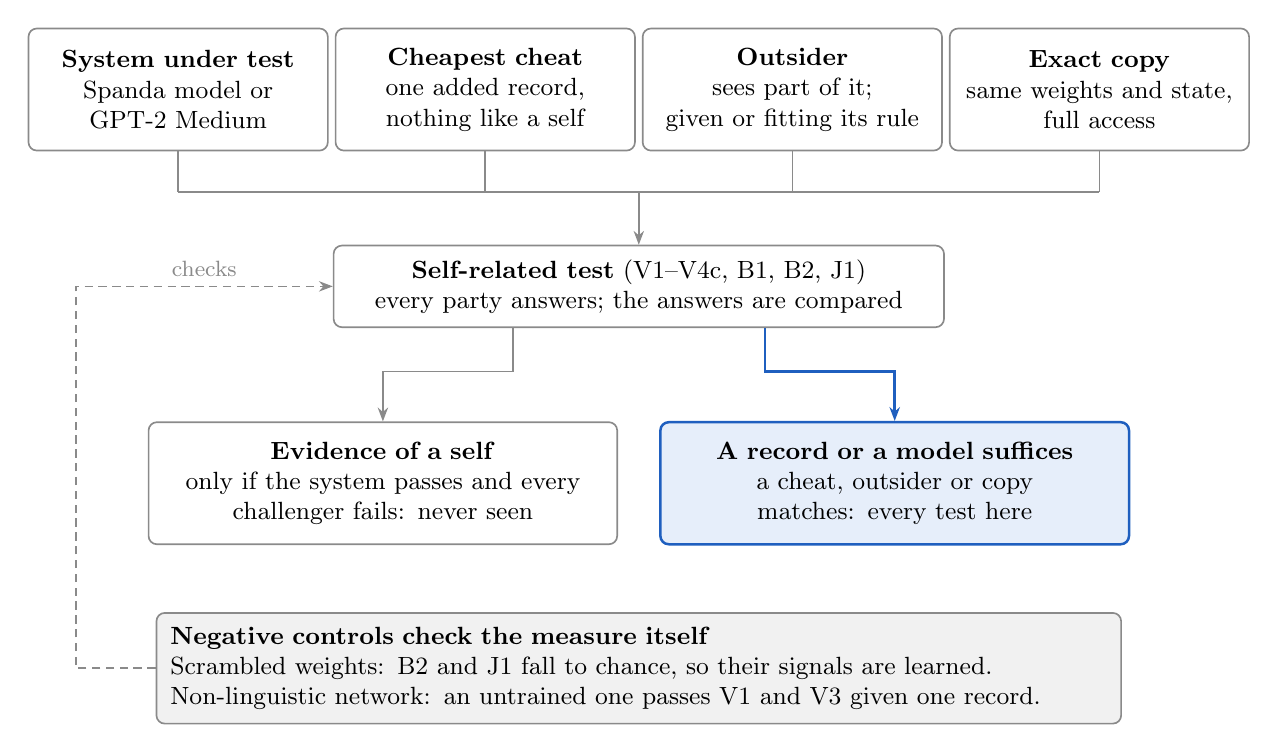
\begin{tikzpicture}[b/.style={box,text width=3.45cm,minimum height=1.55cm}]
\node[b] (s) at (0,0) {\textbf{System under test}\\Spanda model or\\GPT-2 Medium};
\node[b] (c) at (3.9,0) {\textbf{Cheapest cheat}\\one added record,\\nothing like a self};
\node[b] (o) at (7.8,0) {\textbf{Outsider}\\sees part of it;\\given or fitting its rule};
\node[b] (x) at (11.7,0) {\textbf{Exact copy}\\same weights and state,\\full access};
\node[box,text width=7.4cm] (t) at (5.85,-2.5) {\textbf{Self-related test} (V1--V4c, B1, B2, J1)\\every party answers; the answers are compared};
\foreach \n in {s,c,o,x}{\draw[gry,line width=0.6pt] (\n.south) -- (\n.south |- 0,-1.3);}
\draw[gry,line width=0.6pt] (0,-1.3) -- (11.7,-1.3);
\draw[arr] (5.85,-1.3) -- (t.north);
\node[box,text width=5.6cm,minimum height=1.55cm] (e) at (2.6,-5.0) {\textbf{Evidence of a self}\\only if the system passes and every\\challenger fails: never seen};
\node[hl,text width=5.6cm,minimum height=1.55cm] (r) at (9.1,-5.0) {\textbf{A record or a model suffices}\\a cheat, outsider or copy\\matches: every test here};
\draw[arr] ($(t.south)+(-1.6,0)$) -- ($(t.south)+(-1.6,-0.55)$) -| (e.north);
\draw[aarr] ($(t.south)+(1.6,0)$) -- ($(t.south)+(1.6,-0.55)$) -| (r.north);
\node[box,fill=fillg,text width=11.9cm,align=left] (n) at (5.85,-7.35) {\textbf{Negative controls check the measure itself}\\Scrambled weights: B2 and J1 fall to chance, so their signals are learned.\\Non-linguistic network: an untrained one passes V1 and V3 given one record.};
\draw[arr,dash pattern=on 3pt off 2pt] (n.west) -- (-1.3,-7.35) -- (-1.3,-2.5) -- (t.west) node[pos=0.5,above,font=\footnotesize,text=gry]{checks};
\end{tikzpicture}
\end{document}
